\lstset{language={Python2}}

\title{ALPSチュートリアル: Python}

\begin{document}

\begin{frame}
  \titlepage
\end{frame}

\section*{Outline}
\begin{frame}
  \tableofcontents
\end{frame}

\section{データ型}
\begin{frame}[t, fragile]
\frametitle{基本的なデータ型}

\alert{このセクションでは Python で使われる基本的なデータ型を紹介しま
す.} array は numpy モジュールで定義されている型で,Python がもともと持っ
ている型ではありませんが,科学計算では非常に便利な性質を持つので紹介しま
す.

\begin{table}[hb]
 \begin{tabular}{r|l} 
  \textbf{数値}       & int, (long), float, complex \\
  \textbf{文字列}     & 'hello,python' \\
  \textbf{list}       & a = [1, 2, 3] \\
  \textbf{tuple}      & b = (1, 2, 3) \\
  \textbf{dictionary} & c = \{'apple': 100, 'orange': 200, 'pear': 300\} \\
  \textbf{set}        & set([1, 2, 3]) \\
  \textbf{bool}       & True, False \\
  \textbf{array}      & numpy array([1,2,3]) \\
 \end{tabular}
\end{table}

\end{frame}

\begin{frame}[t,fragile]
\frametitle{数値}

整数, 倍精度浮動小数, 複素数の 3 種類あります.
\alert{整数は Python のバージョンで扱いが変わります.}
単精度浮動小数はありません.

\begin{itemize}
 \item int, (long)
       \begin{itemize}
	\item python3 では int,long は int に統合されました.
	\item \alert{python2x と python3x では整数同士の演算で計算結果がちがいます!}

	      python2:  -1/2 = -1, python3: -1/2 = -0.5

       \end{itemize}
 \item float は倍精度のみです.単精度はありません.
 \item complex
       \begin{itemize}
	\item 'j' もしくは 'J' で虚数部を表す 2 + 3j
	\item 実部 real(2+3j) = 2, 虚部 imag(2+3j) = 3  
       \end{itemize}
 \item 型変換を行えます.

       \begin{columns}
	\begin{column}{4cm}
	 \begin{lstlisting}
	  >>> a = 1.8
	  >>> int(a)
	  1
	 \end{lstlisting}	 
	\end{column}
	\begin{column}{4cm}
	 \begin{lstlisting}
	  >>> a = 3
	  >>> float(a)
	  3.0
	 \end{lstlisting}	 
	\end{column}
       \end{columns}
\end{itemize}

\end{frame}

\begin{frame}[t,fragile]
\frametitle{文字列}

\begin{lstlisting}
>>> s = 'ab:cd:ef'   # 文字列の定義
>>> s = s.split(':') # 指定した文字で文字列を分割
>>> print s
['ab', 'cd', 'ef']
>>> '-'.join(s)      # 指定した文字で文字列同士を結合
'ab-cd-ef'
>>> 'a' + 'b' + 'c'  # 文字列を結合
'abc'
\end{lstlisting}

\begin{itemize}
  \item シングルクォートもしくはダブルクォートで囲った文字列で定義できます.
  \item 複数行の文字列は '''...''' もしくは """...""" で囲む
\end{itemize}
\end{frame}

\begin{frame}[t,fragile]
 \frametitle{list, tuple}
 \begin{lstlisting}
  >>>a = [1,2,3,4,5] # list
  >>>a[0]   # インデックスは 0 スタート
  1         # 要素 1 個だけなら返り値はスカラー
  >>>a[2:4] # 2<=,<4 番目のの要素が返される.
  [3,4]     # 複数の要素なら返り値はリスト.
  >>>b = (1,2,3,4,5) # tuple
  >>>b[1:]           # ':' の値を省くこともできる
  (2, 3, 4, 5)
 \end{lstlisting}
 \begin{itemize}
  \item ここではリストの要素として数値のみを扱ったが,python オブジェクトなら何でも リストの要素として扱える
 \end{itemize}
\end{frame}

\begin{frame}[t,fragile]
\frametitle{list のメソッド}
\begin{lstlisting}
>>>a.reverse() # 要素の並びを逆にする
>>>a           # a そのものが変更されるので注意!
[5, 4, 3, 2, 1]
>>>a.pop()  # リストの最後尾の要素を取り出す.
1           # 返り値は取り出された要素
>>>a
[5, 4, 3, 2]
>>>a.sort()
>>>a
[2, 3, 4, 5]
\end{lstlisting}
\begin{itemize}
\item ここではリストの要素として数値のみを扱ったが,python オブジェクトなら何でも リストの要素として扱える
\end{itemize}
\end{frame}




\begin{frame}[t,fragile]
\frametitle{list と tuple の違う点}
\begin{lstlisting}
>>>b = (1)  # これは tuple にならない!
>>>type(b)
int         # 整数扱いになる
>>>b = (1,) # 要素 1 個の tuple を定義する
>>>type(b)
tuple       # これはちゃんと tuple になっている
>>>a = [1]  # これは list
>>>type(a)
list
\end{lstlisting}
\end{frame}

\begin{frame}[t,fragile]
\frametitle{list と tuple の違う点}
\begin{lstlisting}
>>>b += (2, 3, 3)  # 要素を付け加えることはできる
>>>b
(1, 2, 3, 3)
>>>b[3] = 5        # 要素を変更することはできない
Traceback (most recent call last):
  File "<stdin>", line 1, in <module>
TypeError: 'tuple' object does not support item assignment
\end{lstlisting}
\begin{itemize}
\item 要素 1 個の場合の扱いが違う
\item tuple の要素の値は変更できない.
\item tuple は辞書のキーに登録できる.list は不可.
\end{itemize}

\end{frame}

\begin{frame}[t,fragile]
\frametitle{list のコピー}
浅いコピーと深いコピーの 2 種類ある
\begin{columns}
\begin{column}{5cm}
\begin{itemize}
\item 浅いコピーではオブジェクトのアドレスをコピーする
\item 深いコピーではオブジェクトの値をコピーする
\end{itemize}
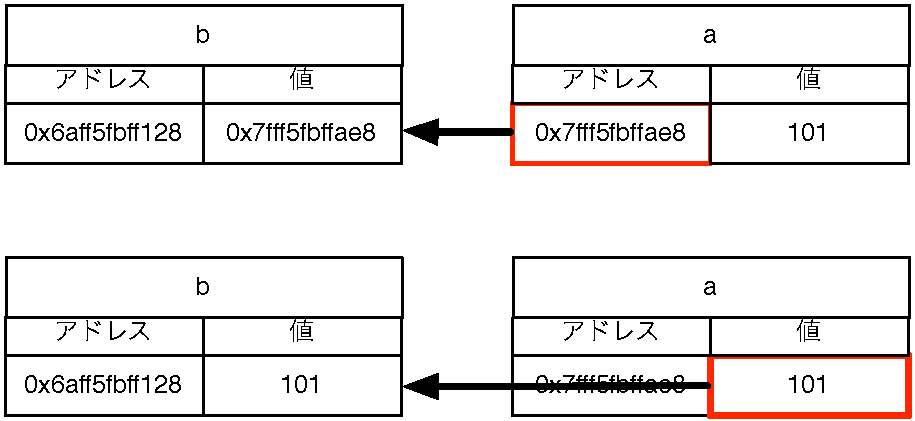
\includegraphics[width = \textwidth]{copy.pdf}
\end{column}

\begin{column}{7cm}
\begin{lstlisting}
>>>a = [101, 102, 103]                 
>>>b = a     # アドレスをコピー
>>>a[1] = 333
>>>print a, b 
[101, 333, 103] [101, 333, 103]
>>>b = a[:]  # 値をコピー
>>>a[1] = 444
>>>print a, b
[101, 444, 103] [101, 333, 103]
\end{lstlisting}
\end{column}
\end{columns}

\end{frame}

\begin{frame}[t,fragile]
\frametitle{ネストされた list のコピー}
\begin{columns}
\begin{column}{6cm}
浅いコピーになってしまう例
\begin{lstlisting}
>>>a = [1, [2, 3]]
>>>b = a[:]
>>>a[0] = 4
>>>a[1][0] = 5
>>>print a, b
[4, [5, 3]] [1, [5, 3]]
>>>
\end{lstlisting}
\end{column}

\begin{column}{6cm}
深いコピー
\begin{lstlisting}
>>>import copy
>>>a = [1, [2, 3]]
>>>b = copy.deepcopy(a)
>>>a[0] = 101
>>>a[1][0] = 102
>>>print a, b
[101, [102, 3]] [1, [2, 3]]
\end{lstlisting}
\end{column}
\end{columns}

\begin{itemize}
\item ネストされているとスライス ':' で返されるのがアドレスになってしまう
\item ネストされた list で深いコピーをするには copy モジュールの deepcopy を使う
\end{itemize}

\end{frame}


\begin{frame}[t,fragile]
\frametitle{辞書型の使い方}
\begin{lstlisting}
>>>dic = {'key0': 0, 'key1': 1}   # key:value の組を登録
>>>dic['key2'] = 2          # key2:2 を登録
>>>dic.keys()               # 辞書に登録されている全ての key
['key2', 'key1', 'key0']
>>>dic.values()             # 全ての val
[2, 1, 0]
>>>dic.items()              # 全ての key:val の組を表示
[('key2', 2), ('key1', 1), ('key0', 0)]  
>>>del dic['key0']          # 辞書から key を削除
>>>dic.items()
[('key2', 2), ('key1', 1)]
\end{lstlisting}

\begin{itemize}
\item 辞書の要素はソートされていない.登録順なども関係ない.
\end{itemize}
\end{frame}

\section{制御フロー}

\begin{frame}[t,fragile]
\frametitle{if-elif-else 文の使い方}
if-elif-else で条件分岐を作れる.
\begin{lstlisting}[stepnumber=1]
>>>if a > 0:
>>>    print '0'
>>>elif a == 0:
>>>    print '1'
>>>else:
>>>    print '2'
>>>
>>>
\end{lstlisting}

三項演算子

\begin{lstlisting}
>>>val = val1 if cond1 else val2
\end{lstlisting}

\end{frame}

\begin{frame}[t,fragile]
\frametitle{for 文の使い方}
\begin{lstlisting}
>>>for i in ('a', 'b', 'c', 'd'):
>>>    print i,    # コンマで改行を抑制している
a b c d
\end{lstlisting}

アンパック代入と enumerate()
\begin{lstlisting}
>>>for i,j in enumerate(('a', 'b', 'c', 'd')):
>>>    print i, j
0 a
1 b
...
\end{lstlisting}
アンパック代入は python で使える一般的なテクニックです.
\begin{lstlisting}
>>>i,j,k = ['a', 'b', 'c']
\end{lstlisting}
\end{frame}

\begin{frame}[t,fragile]
\frametitle{while 文の使い方}
\begin{lstlisting}
a = 0
while a in range(10):
    a += 1
    if a < 3:
        continue
    elif a == 8:
        break
    print a

\end{lstlisting}

\begin{itemize}
\item カレントディレクトリに上の内容で exWhile.py というファイルを作って import してみましょう
\item "val in シークエンス:" というフレーズは while だけでなく if, for など至る所で使えます
\item continue, break も同じく if, for などでも使えます
\end{itemize}

\end{frame}
\section{関数}
\begin{frame}[t,fragile]
\frametitle{関数}
\begin{lstlisting}
>>> def f(x, y):
>>> ....z = x * y  # 空白 4 つのインデント!
>>> ....for i in [1, 2, 3]:
>>> ....    z += i
>>> ....return z
>>>
>>> f(2,3)
12
\end{lstlisting}
\begin{itemize}
\item def 関数名(変数,...): で関数が定義できます
\item Python ではインデント (空白4つ) によりスコープを制御します
\end{itemize}
\end{frame}

\section{モジュール}
\begin{frame}[t]
\frametitle{Python プログラムの階層構造}
\begin{itemize}
\item プログラムファイルのディレクトリ構成 == 名前空間
\item モジュール
\begin{itemize}
 \item 1 つの "hoge.py" ファイルが 1 つのモジュール
\end{itemize}
\item パッケージ
\end{itemize}
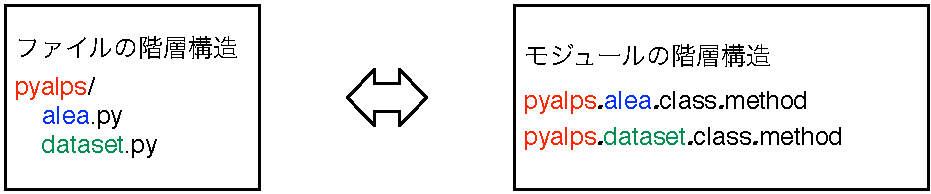
\includegraphics[width=\textwidth]{module.pdf}
\end{frame}

\begin{frame}[t,fragile]
\frametitle{モジュールの読み込み}
\begin{lstlisting}
>>> import fff as f    # 別名をつけてインポート
>>> f.ggg(x, y)
...
>>> from fff import *  # fff 以下のすべてをインポート
>>> ggg(x, y)          # 名前空間 fff が外れる
...
>>> from fff import ggg as g # ggg のみを指定してインポート
>>> g(x, y)
\end{lstlisting}
\begin{itemize}
\item fff モジュール中の ggg 関数を呼び出しています.
\item 呼び出し方により名前空間の階層が変わっています.
\end{itemize}

\end{frame}

\section{ファイルの読み書き}
\begin{frame}[t,fragile]
\frametitle{ファイルの読み書き}
\begin{columns}
\begin{column}{8cm}
ファイルから1行ごとにデータを読み込む方法
\begin{lstlisting}
for line in open('dat.txt', 'r'):
    items = line.split('')
    print items[0], float(items[1])
\end{lstlisting}
\end{column}
\begin{column}{4cm}
入力データ (dat.txt)
\begin{lstlisting}
a 3.432
b 1.42
c 2.159
\end{lstlisting}
\end{column}
\end{columns}

\begin{itemize}
\item open で dat.txt ファイルを readonly で読み込む
\item 読み込んだファイルを 1 行毎に処理する.読み込まれた行は 1 つのス
      トリングとして扱われるので区切り文字(今の場合空白)で分割してい
      る.
\item 読み込んだストリングを浮動小数点にキャストしている.
\end{itemize}
上の例では for 文の終了とともにファイルは自動で閉じられる.しかし,一般的には
\begin{itemize}
\item f = open('dat.txt', 'r') として読み込んだ場合,ファイルを読み終
      えたら f.close() で閉じなければならない.
\end{itemize}
\end{frame}

\section{参考サイト}
\begin{frame}[t]
\frametitle{参考サイト}
\begin{itemize}
\item 科学技術計算のために python を始めよう
      \url{http://www.ike-dyn.ritsumei.ac.jp/~uchida/scipy-lecture-notes/intro/index.html}
\item 初心者のはまりどころ \url{http://webtech-walker.com/archive/2010/10/13191417.html}
\item Doug Hellmannさん \url{http://doughellmann.com}
      \begin{itemize}
      \item 標準モジュールなどの使い方が例とともに書いてあり分かりやすい
      \end{itemize}
\end{itemize}

\end{frame}


\end{document}
